\documentclass[aspectratio=169, 10pt]{beamer}

% ─── Theme & Colour ───────────────────────────────────────────────────────────
\usetheme{Madrid}
\usecolortheme{seahorse}
\setbeamertemplate{navigation symbols}{}
\setbeamertemplate{footline}[frame number]

\definecolor{primaryblue}{RGB}{25, 60, 120}
\definecolor{accentorange}{RGB}{220, 100, 30}
\definecolor{lightgray}{RGB}{240, 240, 245}
\definecolor{darkgray}{RGB}{80, 80, 80}
\definecolor{codegreen}{RGB}{0, 120, 80}

\setbeamercolor{title}{fg=white, bg=primaryblue}
\setbeamercolor{frametitle}{fg=white, bg=primaryblue}
\setbeamercolor{block title}{fg=white, bg=primaryblue}
\setbeamercolor{block body}{bg=lightgray}
\setbeamercolor{alerted text}{fg=accentorange}
\setbeamercolor{structure}{fg=primaryblue}

% ─── Packages ─────────────────────────────────────────────────────────────────
\usepackage{tikz}
\usetikzlibrary{arrows.meta, positioning, shapes.geometric, fit, backgrounds}
\usepackage{booktabs}
\usepackage{colortbl}
\usepackage{listings}
\usepackage{amsmath}
\usepackage{xcolor}
\usepackage{multirow}
\usepackage{array}
\usepackage{graphicx}
\usepackage{pifont}

% ─── Simple Icon Macros (replacement for fontawesome5) ───────────────────────
\newcommand{\faChartBar}{\ding{111}\ }
\newcommand{\faMicroscope}{$\bigcirc$\ }
\newcommand{\faExclamationTriangle}{\ding{72}\ }
\newcommand{\faLightbulb}{\ding{78}\ }
\newcommand{\faDatabase}{[DB]\ }
\newcommand{\faCogs}{[*]\ }
\newcommand{\faChartLine}{[\#]\ }

\lstset{
  basicstyle=\ttfamily\scriptsize,
  keywordstyle=\color{primaryblue}\bfseries,
  commentstyle=\color{darkgray}\itshape,
  stringstyle=\color{codegreen},
  backgroundcolor=\color{lightgray},
  frame=single,
  framerule=0.4pt,
  rulecolor=\color{primaryblue},
  breaklines=true,
  showstringspaces=false
}

% ─── Title Information ────────────────────────────────────────────────────────
\title[No-Pos Transformer]{%
  \textbf{Transformer Language Models}\\
  \textit{Without Positional Encodings Still Learn Positional Information}%
}
\subtitle{Deep Learning Foundations --- AI21204 (Graduate Course Project)}
\author[Patra et al.]{%
  Kingshuk Patra \and Shubhajeet Das \and Ibtesam Ahmed \\
  Aditya Mondal \and Abhishek Kumar%
}
\date{\today}
\institute[AI21204]{Graduate Course Project}

% ─── Document ─────────────────────────────────────────────────────────────────
\begin{document}

% ── Title Slide ───────────────────────────────────────────────────────────────
\begin{frame}[plain]
  \titlepage
\end{frame}

% ── Table of Contents ─────────────────────────────────────────────────────────
\begin{frame}{Outline}
  \tableofcontents[hideallsubsections]
\end{frame}

% ══════════════════════════════════════════════════════════════════════════════
\section{Motivation \& Research Question}
% ══════════════════════════════════════════════════════════════════════════════

\begin{frame}{Motivation}
  \begin{columns}[T]
    \begin{column}{0.55\textwidth}
      \begin{block}{Core Question}
        \textit{Do Transformers \textbf{require} explicit positional encodings, or do they
        implicitly learn positional information even without them?}
      \end{block}
      \vspace{0.5em}
      \begin{itemize}
        \item Positional encodings are considered \alert{essential} in standard Transformer design
        \item Recent work suggests models may self-organize positional representations
        \item This project \textbf{replicates and extends} the paper:\\
              \textit{``Transformer Language Models without Positional Encodings
              Still Learn Positional Information''}
      \end{itemize}
    \end{column}
    \begin{column}{0.42\textwidth}
      \begin{alertblock}{What We Measure}
        \begin{enumerate}
          \item \textbf{Language modelling quality} via perplexity on WikiText-103
          \item \textbf{Implicit positional encoding} via layer-wise linear-regression probing (MAE)
        \end{enumerate}
      \end{alertblock}
      \vspace{0.5em}
      \begin{block}{Our Variants}
        \begin{itemize}
          \item \textbf{NoPos} — no encoding
          \item \textbf{Sinusoidal} — fixed
          \item \textbf{Learned} — trainable
          \item \textbf{ALiBi} — bias-based
        \end{itemize}
      \end{block}
    \end{column}
  \end{columns}
\end{frame}

% ══════════════════════════════════════════════════════════════════════════════
\section{Dataset \& Preprocessing}
% ══════════════════════════════════════════════════════════════════════════════

\begin{frame}{Dataset: WikiText-103}
  \begin{columns}[T]
    \begin{column}{0.48\textwidth}
      \begin{block}{Dataset Facts}
        \begin{tabular}{ll}
          \toprule
          \textbf{Property} & \textbf{Value} \\
          \midrule
          Corpus & Wikipedia articles \\
          Size   & 314M tokens \\
          Source & HuggingFace Hub \\
          \midrule
          \textbf{Split} & \textbf{Examples} \\
          \midrule
          Train      & $\sim$1.8M \\
          Validation & $\sim$3.7K \\
          Test       & $\sim$4.3K \\
          \bottomrule
        \end{tabular}
      \end{block}
    \end{column}
    \begin{column}{0.5\textwidth}
      \begin{block}{Preprocessing Pipeline}
        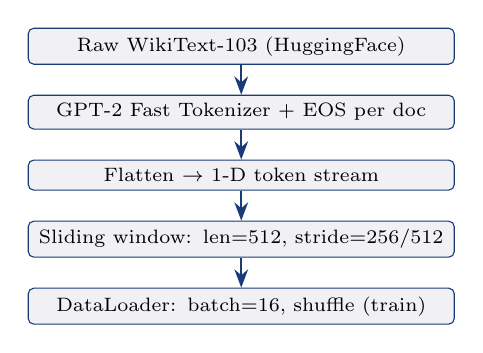
\begin{tikzpicture}[
            node distance=0.38cm,
            box/.style={draw=primaryblue, rounded corners=2pt, fill=lightgray,
                        font=\scriptsize, text width=5.2cm, align=center, inner sep=3pt},
            arr/.style={-Stealth, thick, color=primaryblue}
          ]
          \node[box] (raw)  {Raw WikiText-103 (HuggingFace)};
          \node[box] (tok)  [below=of raw]  {GPT-2 Fast Tokenizer + EOS per doc};
          \node[box] (flat) [below=of tok]  {Flatten $\to$ 1-D token stream};
          \node[box] (seq)  [below=of flat] {Sliding window: len=512, stride=256/512};
          \node[box] (bat)  [below=of seq]  {DataLoader: batch=16, shuffle (train)};
          \draw[arr] (raw)--(tok);
          \draw[arr] (tok)--(flat);
          \draw[arr] (flat)--(seq);
          \draw[arr] (seq)--(bat);
        \end{tikzpicture}
      \end{block}
    \end{column}
  \end{columns}
  \vspace{0.3em}
  \begin{alertblock}{Teacher Forcing Format}
    \textbf{x} = \texttt{tokens[i : i+512]}, \quad
    \textbf{y} = \texttt{tokens[i+1 : i+513]} \quad (shifted by 1)
  \end{alertblock}
\end{frame}

% ══════════════════════════════════════════════════════════════════════════════
\section{Model Architecture}
% ══════════════════════════════════════════════════════════════════════════════

\begin{frame}{Model Architecture: \texttt{CausalTransformerLM}}
  \begin{columns}[T]
    \begin{column}{0.5\textwidth}
      \begin{block}{Overall Architecture}
        \begin{enumerate}
          \item \textbf{Token Embedding} \hfill $\mathbb{R}^{B \times T \times d}$
          \item \textbf{Positional Signal} (variant-dependent)
          \item \textbf{8 $\times$ TransformerBlock}
          \begin{itemize}
            \item Pre-LN \& Causal Self-Attention
            \item Feed-Forward (4$d$ hidden, GELU)
          \end{itemize}
          \item \textbf{Final LayerNorm}
          \item \textbf{LM Head} \hfill $\mathbb{R}^{B \times T \times |V|}$
        \end{enumerate}
      \end{block}
      \begin{block}{Key Design Choices}
        \begin{itemize}
          \item \alert{Weight tying:} \texttt{lm\_head.weight = tok\_emb.weight}\\
                saves $\approx$26M parameters
          \item \textbf{Return hidden states:} optional flag collects all layer outputs
                for probing
          \item Causal mask: upper-triangular $-\infty$ before softmax
        \end{itemize}
      \end{block}
    \end{column}
    \begin{column}{0.48\textwidth}
      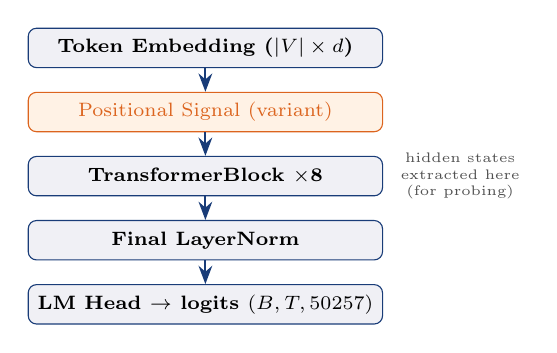
\begin{tikzpicture}[
          node distance=0.3cm,
          layer/.style={draw=primaryblue, fill=lightgray, rounded corners=3pt,
                        minimum width=4.5cm, minimum height=0.5cm,
                        font=\scriptsize\bfseries, align=center},
          posbox/.style={draw=accentorange, fill=orange!10, rounded corners=3pt,
                         minimum width=4.5cm, minimum height=0.5cm,
                         font=\scriptsize, align=center},
          arr/.style={-Stealth, thick, color=primaryblue}
        ]
        \node[layer] (emb)  {Token Embedding ($|V| \times d$)};
        \node[posbox] (pos)  [below=of emb] {\textcolor{accentorange}{Positional Signal (variant)}};
        \node[layer] (b1)   [below=of pos] {TransformerBlock $\times$8};
        \node[layer] (ln)   [below=of b1]  {Final LayerNorm};
        \node[layer] (head) [below=of ln]  {LM Head $\to$ logits $(B, T, 50257)$};
        \draw[arr] (emb)--(pos);
        \draw[arr] (pos)--(b1);
        \draw[arr] (b1)--(ln);
        \draw[arr] (ln)--(head);
        \node[font=\tiny, color=darkgray, right=0.1cm of b1, align=center]
      {hidden states\\extracted here\\(for probing)};
      \end{tikzpicture}
    \end{column}
  \end{columns}
\end{frame}

\begin{frame}{Four Positional Encoding Variants}
  \begin{block}{}
    \small
    \centering
    \begin{tabular}{p{2.2cm}p{4.5cm}p{5.5cm}}
      \toprule
      \textbf{Variant} & \textbf{Mechanism} & \textbf{Key Properties} \\
      \midrule
      NoPos &
        No positional signal applied &
        Embeddings fed directly to blocks; probes test if position is \textit{implicitly} learned \\[0.5em]
      Sinusoidal &
        Fixed $\sin$/$\cos$ at exponentially spaced frequencies (Vaswani et al.\ 2017) &
        Non-trainable; pre-computed buffer; deterministic \\[0.5em]
      Learned &
        Trainable \texttt{nn.Embedding(max\_len, d)} &
        One learned vector per position; flexible but fixed to training length \\[0.5em]
      ALiBi &
        Subtract head-specific linear bias $-m \cdot |i - j|$ from attention logits &
        No embedding added; enables length extrapolation; slopes follow geometric schedule \\
      \bottomrule
    \end{tabular}
  \end{block}
  \vspace{0.4em}
  \begin{columns}
    \begin{column}{0.5\textwidth}
      \begin{block}{ALiBi Slope Schedule}
        \[
          m_k = 2^{-8k / n_{\text{heads}}}, \quad k = 1,\ldots,n_{\text{heads}}
        \]
        Non-power-of-2 heads handled via interpolation.
      \end{block}
    \end{column}
    \begin{column}{0.48\textwidth}
      \begin{block}{Sinusoidal Formula}
        \[
          \text{PE}_{(p,2i)} = \sin\!\left(\frac{p}{10000^{2i/d}}\right), \quad
          \text{PE}_{(p,2i+1)} = \cos\!\left(\frac{p}{10000^{2i/d}}\right)
        \]
      \end{block}
    \end{column}
  \end{columns}
\end{frame}

% ══════════════════════════════════════════════════════════════════════════════
\section{Training Pipeline}
% ══════════════════════════════════════════════════════════════════════════════

\begin{frame}{Training Pipeline}
  \begin{columns}[T]
    \begin{column}{0.52\textwidth}
      \begin{block}{Optimisation Setup}
        \begin{tabular}{ll}
          \toprule
          \textbf{Component}     & \textbf{Setting} \\
          \midrule
          Loss        & Cross-entropy (token-avg.) \\
          Optimiser   & AdamW, lr = $3\times10^{-4}$ \\
          Weight decay & 0.01 \\
          LR schedule  & Cosine + linear warmup\\
          Warmup steps & 500 \\
          Grad clipping & max norm = 1.0 \\
          Precision    & AMP (FP16 / FP32) \\
          Epochs (local) & 200 \\
          Epochs (Kaggle) & 3 \\
          \bottomrule
        \end{tabular}
      \end{block}
      \begin{block}{Gradient Accumulation}
        Micro-batches summed for $G$ steps:\\
        $\mathcal{L}_{\text{accum}} = \frac{1}{G}\sum_{g=1}^{G}\mathcal{L}_g$\\
        Enables larger effective batch size on limited VRAM.
      \end{block}
    \end{column}
    \begin{column}{0.46\textwidth}
      \begin{block}{Per-Epoch Loop}
        \begin{tikzpicture}[
            node distance=0.32cm,
            step/.style={draw=primaryblue, fill=lightgray, rounded corners=2pt,
                         font=\scriptsize, text width=4.1cm, align=left, inner sep=3pt},
            arr/.style={-Stealth, thick, color=primaryblue}
          ]
          \node[step] (fwd) {\textbf{Forward:} logits = model(x)};
          \node[step] (loss)[below=of fwd] {\textbf{Loss:} CE(logits, y) / G};
          \node[step] (bwd) [below=of loss]{\textbf{Backward:} scaler.scale(loss).backward()};
          \node[step] (opt) [below=of bwd] {\textbf{Step (every G):} clip $\to$ AdamW $\to$ scheduler};
          \node[step] (val) [below=of opt] {\textbf{Validation:} val\_loss, val\_ppl};
          \node[step] (ckpt)[below=of val] {\textbf{Checkpoint:} last.pt + best.pt};
          \draw[arr](fwd)--(loss);\draw[arr](loss)--(bwd);
          \draw[arr](bwd)--(opt);\draw[arr](opt)--(val);
          \draw[arr](val)--(ckpt);
        \end{tikzpicture}
      \end{block}
    \end{column}
  \end{columns}
\end{frame}

% ══════════════════════════════════════════════════════════════════════════════
\section{Evaluation \& Probing}
% ══════════════════════════════════════════════════════════════════════════════

\begin{frame}{Dual Evaluation Pipeline}
  \begin{columns}[T]
    \begin{column}{0.48\textwidth}
      \begin{block}{\faChartBar Standard Metrics}
        \begin{itemize}
          \item Load \texttt{best.pt} checkpoint
          \item Run model on test/val split (\texttt{no\_grad})
          \item \textbf{Average cross-entropy loss} over all tokens
          \item \textbf{Perplexity:} $\text{PPL} = e^{\mathcal{L}}$
          \item Lower PPL $\Rightarrow$ better language model
        \end{itemize}
      \end{block}
      \vspace{0.4em}
      \begin{alertblock}{\faMicroscope Layerwise Probing (Key)}
        For each Transformer layer $l \in \{0, \ldots, L+1\}$:
        \begin{enumerate}
          \item Collect $\mathbf{X}_l \in \mathbb{R}^{N\cdot T \times d}$
          \item Build augmented matrix $\tilde{\mathbf{X}} = [\mathbf{X}_l \mid \mathbf{1}]$
          \item Solve: $\tilde{\mathbf{X}}\,\mathbf{w} \approx \mathbf{y}$ (least squares)
          \item Compute \textbf{MAE} = $\frac{1}{NT}\|\hat{\mathbf{y}} - \mathbf{y}\|_1$
        \end{enumerate}
        \textbf{Lower MAE} $\Rightarrow$ stronger positional signal at layer $l$
      \end{alertblock}
    \end{column}
    \begin{column}{0.50\textwidth}
      \begin{block}{Why Layerwise Probing?}
        \begin{itemize}
          \item \textbf{NoPos} has no explicit signal — probing tests \textit{implicit} learning
          \item Reveals \textit{where} in the network positional information emerges
          \item Linear probe = minimal model $\Rightarrow$ tests \textbf{representation quality},
                not probe capacity
          \item Uses closed-form \texttt{torch.linalg.lstsq} (efficient, exact)
        \end{itemize}
      \end{block}
      \vspace{0.3em}
      \begin{block}{Layers Probed}
        \begin{center}
        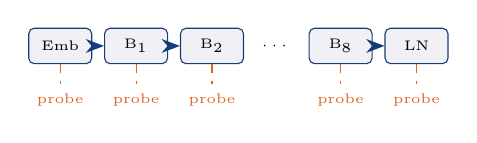
\begin{tikzpicture}[
            b/.style={draw=primaryblue, fill=lightgray, rounded corners=2pt,
                      font=\tiny, minimum width=0.8cm, minimum height=0.45cm},
            a/.style={-Stealth, thick, color=primaryblue}
          ]
          \node[b] (l0) {Emb};
          \node[b] (l1) [right=0.15cm of l0] {B$_1$};
          \node[b] (l2) [right=0.15cm of l1] {B$_2$};
          \node[font=\tiny] (dots) [right=0.1cm of l2] {$\cdots$};
          \node[b] (l8) [right=0.1cm of dots] {B$_8$};
          \node[b] (lf) [right=0.15cm of l8] {LN};
          \draw[a](l0)--(l1);\draw[a](l1)--(l2);\draw[a](l8)--(lf);
          \foreach \n in {l0,l1,l2,l8,lf}
            \draw[-,dashed,accentorange] (\n.south)--++(0,-0.25)
              node[font=\tiny,accentorange,below] {probe};
        \end{tikzpicture}
        \end{center}
        10 probing points: embedding + 8 blocks + post-LN
      \end{block}
    \end{column}
  \end{columns}
\end{frame}

% ══════════════════════════════════════════════════════════════════════════════
\section{System Design}
% ══════════════════════════════════════════════════════════════════════════════

\begin{frame}{System Architecture}
  \begin{columns}[T]
    \begin{column}{0.5\textwidth}
      \begin{block}{Module Responsibilities}
        \begin{tabular}{>{\scriptsize}lp{5.1cm}}
          \toprule
          \normalfont\textbf{Module} & \textbf{Role} \\
          \midrule
          \texttt{config.py}    & YAML $\to$ typed dataclasses \\
          \texttt{data.py}      & Download, tokenise, chunk, batch \\
          \texttt{positional.py} & All 4 PE strategies + attention \\
          \texttt{model.py}     & Assemble \texttt{CausalTransformerLM} \\
          \texttt{train.py}     & AMP loop, checkpointing, scheduler \\
          \texttt{evaluate.py}  & PPL + layerwise linear probing \\
          \texttt{generation.py} & Top-k / temperature sampling \\
          \texttt{utils.py}     & Seeds, devices, logging, metrics \\
          \texttt{compare.py}   & Run all 4 variants sequentially \\
          \bottomrule
        \end{tabular}
      \end{block}
    \end{column}
    \begin{column}{0.48\textwidth}
      \begin{block}{Design Patterns Used}
        \begin{description}
          \item[\alert{Strategy}] \texttt{pos\_encoding} string enum selects PE at init
          \item[\alert{Dataclass Config}] Nested typed configs with recursive YAML merge
          \item[\alert{Template Hook}] \texttt{return\_hidden\_states} flag activates probing path
          \item[\alert{Factory}] \texttt{build\_optimizer}, \texttt{build\_scheduler}
          \item[\alert{Weight Tying}] Shared embedding \& LM head ($-$26M params)
        \end{description}
      \end{block}
      \begin{block}{Output Artefacts}
        \begin{itemize}
          \item \texttt{runs/<exp>/config.json}
          \item \texttt{runs/<exp>/train.log}
          \item \texttt{runs/<exp>/history.json}
          \item \texttt{runs/<exp>/checkpoints/best.pt}
          \item \texttt{runs/<exp>/checkpoints/last.pt}
        \end{itemize}
      \end{block}
    \end{column}
  \end{columns}
\end{frame}

\begin{frame}{Text Generation Pipeline}
  \begin{block}{Autoregressive Sampling (\texttt{generation.py})}
    \begin{columns}[T]
      \begin{column}{0.55\textwidth}
        \begin{tikzpicture}[
            node distance=0.32cm,
            step/.style={draw=primaryblue, fill=lightgray, rounded corners=2pt,
                         font=\scriptsize, text width=5.0cm, align=left, inner sep=3pt},
            arr/.style={-Stealth, thick, color=primaryblue}
          ]
          \node[step] (p) {Tokenise prompt $\to$ \texttt{input\_ids} $(1, L)$};
          \node[step] (f) [below=of p] {Forward pass $\to$ logits $(1, T, |V|)$};
          \node[step] (l) [below=of f] {Take last-token logits: $[:, -1, :]$};
          \node[step] (t) [below=of l] {Divide by temperature $\tau$};
          \node[step] (k) [below=of t] {Top-$k$ filter: zero out all but top $k$};
          \node[step] (s) [below=of k] {Softmax $\to$ sample $\to$ append token};
          \draw[arr](p)--(f);\draw[arr](f)--(l);\draw[arr](l)--(t);
          \draw[arr](t)--(k);\draw[arr](k)--(s);
          \draw[->,thick,accentorange] (s.east) -- ++(0.3,0) -- ++(0,1.8)
            -- (f.east) node[midway,right,font=\tiny\color{accentorange}]{repeat};
        \end{tikzpicture}
      \end{column}
      \begin{column}{0.42\textwidth}
        \begin{alertblock}{Temperature Control}
          \begin{itemize}
            \item $\tau = 0$ : greedy (argmax)
            \item $\tau = 1$ : standard softmax
            \item $\tau > 1$ : flatter (more random)
          \end{itemize}
        \end{alertblock}
        \vspace{0.4em}
        \begin{block}{Example}
          \textbf{Prompt:} ``The theory of''\\[0.3em]
          \textbf{Output:} ``The theory of knowledge and belief is a central concern
          of epistemology \ldots''
        \end{block}
      \end{column}
    \end{columns}
  \end{block}
\end{frame}

% ══════════════════════════════════════════════════════════════════════════════
\section{Dependencies \& Technical Details}
% ══════════════════════════════════════════════════════════════════════════════

\begin{frame}{Dependencies \& Project Stats}
  \begin{columns}[T]
    \begin{column}{0.52\textwidth}
      \begin{block}{Key Dependencies}
        \begin{tabular}{llp{3.0cm}}
          \toprule
          \textbf{Library} & \textbf{Version} & \textbf{Role} \\
          \midrule
          PyTorch      & $\geq$2.1.0 & Core DL framework \\
          Transformers & $\geq$5.5.4 & GPT-2 tokeniser \\
          Datasets     & $\geq$4.8.4 & WikiText-103 loader \\
          NumPy        & $\geq$2.4.4 & Token array handling \\
          PyYAML       & $\geq$6.0.3 & Config parsing \\
          tqdm         & $\geq$4.67.3 & Training progress bars \\
          matplotlib   & $\geq$3.10.8 & Result visualisation \\
          pandas       & $\geq$3.0.2  & Notebook analysis \\
          \bottomrule
        \end{tabular}
      \end{block}
    \end{column}
    \begin{column}{0.46\textwidth}
      \begin{block}{Project Statistics}
        \begin{tabular}{ll}
          \toprule
          \textbf{Metric}       & \textbf{Value} \\
          \midrule
          Language         & Python 3.12 \\
          Python modules   & 13 \\
          YAML configs     & 6 \\
          Lines of code    & $\approx$1,000 \\
          YAML lines       & $\approx$220 \\
          Vocab size       & 50,257 (GPT-2) \\
          Transformer depth & 8 blocks \\
          Sequence length  & 512 tokens \\
          Batch size       & 16 \\
          \bottomrule
        \end{tabular}
      \end{block}
      \begin{alertblock}{Reproducibility}
        \texttt{seed\_everything()} sets seeds for \texttt{random}, \texttt{numpy},
        \texttt{torch}, and \texttt{torch.cuda} at the start of every run.
        Dependency versions are locked via \texttt{uv} lockfile.
      \end{alertblock}
    \end{column}
  \end{columns}
\end{frame}

% ══════════════════════════════════════════════════════════════════════════════

% ══════════════════════════════════════════════════════════════════════════════
\section{Summary}
% ══════════════════════════════════════════════════════════════════════════════

\begin{frame}{Summary}
  \begin{block}{What We Built}
    A \textbf{research replication system} in Python 3.12 + PyTorch + HuggingFace that:
    \begin{enumerate}
      \item Trains four Transformer positional-encoding variants on WikiText-103
      \item Measures language modelling quality via \textbf{perplexity}
      \item Quantifies implicit positional representations via \textbf{layer-wise linear probing (MAE)}
    \end{enumerate}
  \end{block}
  \vspace{0.5em}
  \begin{columns}
    \begin{column}{0.32\textwidth}
      \begin{block}{\faDatabase Data}
        WikiText-103\\
        314M tokens\\
        GPT-2 tokeniser\\
        512-token windows
      \end{block}
    \end{column}
    \begin{column}{0.32\textwidth}
      \begin{block}{\faCogs Models}
        4 PE variants\\
        8-layer Transformer\\
        AMP + AdamW\\
        Cosine LR schedule
      \end{block}
    \end{column}
    \begin{column}{0.32\textwidth}
      \begin{block}{\faChartLine Analysis}
        PPL benchmarking\\
        10-layer MAE probing\\
        Least-squares regression\\
        Notebook visualisation
      \end{block}
    \end{column}
  \end{columns}
  \vspace{0.8em}
  \begin{center}
    \Large\textbf{\textit{Even without explicit positional encodings,\\
    Transformers learn to represent token positions.}}
  \end{center}
\end{frame}

% ── Questions ─────────────────────────────────────────────────────────────────
\begin{frame}[plain]
  \begin{center}
    \vspace{1.5cm}
    {\Huge \textbf{Thank You}}\\[1em]
    {\large Questions \& Discussion}\\[2em]
    \begin{tabular}{c}
      Kingshuk Patra \quad Shubhajeet Das \quad Ibtesam Ahmed \\[0.3em]
      Aditya Mondal \quad Abhishek Kumar
    \end{tabular}\\[1.5em]
    {\small Deep Learning Foundations --- AI21204}
  \end{center}
\end{frame}

\end{document}